% ============================================================
% บทที่ 2: ระบบนิเวศเซนเซอร์เกษตรและสะพานเชื่อมต่ออุตสาหกรรม RS485 Modbus
% ============================================================
\chapter[ระบบนิเวศเซนเซอร์เกษตรและสะพานเชื่อมต่ออุตสาหกรรม RS485 Modbus]{ระบบนิเวศเซนเซอร์เกษตร\\และสะพานเชื่อมต่ออุตสาหกรรม RS485 Modbus}
\label{chap:ch02}

% ------------------------------------------------------------
% แผนบริหารการสอนประจำบทที่ 2 (หน้า 1/2)
% ------------------------------------------------------------
\section*{แผนบริหารการสอนประจำบทที่ 2}
\addcontentsline{toc}{section}{แผนบริหารการสอนประจำบทที่ 2}

\begin{planbox}{หัวข้อเนื้อหาประจำบท}
\begin{enumerate}[topsep=1pt, itemsep=0.5pt, partopsep=0pt, parsep=0pt, leftmargin=1.5em]
    \item สรีรวิทยาของพืชและการตรวจวัดสภาพแวดล้อมทางฟิสิกส์ในดินและบรรยากาศ
    \item เซนเซอร์ตรวจวัดดินแบบหลายพารามิเตอร์ ความชื้น อุณหภูมิ การนำไฟฟ้า และธาตุอาหาร NPK
    \item การตรวจวัดสภาวะภูมิอากาศจุลภาค อุณหภูมิ ความชื้นสัมพัทธ์ และรังสีสังเคราะห์แสง PAR
    \item สถาปัตยกรรมสะพานสื่อสารเชื่อมต่อมาตรฐานอุตสาหกรรม RS485 Modbus RTU สู่ Zigbee
    \item การวิเคราะห์เปรียบเทียบระหว่างโหนดเซนเซอร์เชิงพาณิชย์และฮาร์ดแวร์โอเพนซอร์สแบบกำหนดเอง
\end{enumerate}
\end{planbox}

\begin{planbox}{วัตถุประสงค์เชิงพฤติกรรม}
\begin{enumerate}[topsep=1pt, itemsep=0.5pt, partopsep=0pt, parsep=0pt, leftmargin=1.5em]
    \item อธิบายหลักการทำงานของหัววัดความชื้นดินแบบความจุไฟฟ้าและการนำไฟฟ้าได้อย่างถูกต้อง
    \item เชื่อมต่อและสื่อสารกับเซนเซอร์อุตสาหกรรมผ่านโพรโทคอล Modbus RTU ได้อย่างสมบูรณ์
    \item ออกแบบวงจรสะพานสื่อสาร RS485 ร่วมกับโมดูลไมโครคอนโทรลเลอร์ Zigbee ได้
    \item คำนวณและปรับเทียบค่าความถูกต้องของข้อมูลเซนเซอร์ทางการเกษตรได้อย่างเป็นระบบ
    \item ประเมินความคุ้มค่าและความเหมาะสมระหว่างการจัดซื้ออุปกรณ์สำเร็จรูปและการพัฒนาขึ้นเองได้
\end{enumerate}
\end{planbox}

\newpage

% ------------------------------------------------------------
% แผนบริหารการสอนประจำบทที่ 2 (หน้า 2/2)
% ------------------------------------------------------------
\begin{planbox}{วิธีสอนและกิจกรรมการเรียนการสอน}
\begin{enumerate}[topsep=1pt, itemsep=0.5pt, partopsep=0pt, parsep=0pt, leftmargin=1.5em]
    \item การบรรยายหลักการฟิสิกส์ของหัววัดเซนเซอร์ดินและเซนเซอร์ทางแสง
    \item การสาธิตการต่อวงจรและส่งคำสั่งอ่านค่ารีจิสเตอร์ Modbus RTU ด้วยโปรแกรมทดสอบ
    \item การฝึกปฏิบัติการต่อสายโพรบ 7-in-1 ร่วมกับไอซีแปลงสัญญาณ MAX485 และโหนด Zigbee
    \item การทดลองปรับเทียบค่า EC และ pH ด้วยสารละลายมาตรฐานในห้องปฏิบัติการ
    \item การอภิปรายเปรียบเทียบคุณสมบัติเชิงเทคนิคและงบประมาณการลงทุนในแปลงจริง
\end{enumerate}
\end{planbox}

\begin{planbox}{สื่อการเรียนการสอน}
\begin{enumerate}[topsep=1pt, itemsep=0.5pt, partopsep=0pt, parsep=0pt, leftmargin=1.5em]
    \item เอกสารประกอบการสอนวิชาระบบเซนเซอร์และเครื่องมือวัดทางการเกษตร
    \item หัววัดเซนเซอร์ดินอุตสาหกรรม RS485 ชนิด 7-in-1 โพรบสแตนเลสสตีลมาตรฐาน IP68
    \item เซนเซอร์อุณหภูมิและความชื้น SHT30 หัวครอบโลหะเผา และเซนเซอร์วัดแสง BH1750
    \item โมดูลแปลงระดับสัญญาณ TTL เป็น RS485 พร้อมวงจรแยกสัญญาณกัลวานิก
    \item สารละลายมาตรฐานสำหรับการปรับเทียบค่าการนำไฟฟ้าและกรดด่าง
\end{enumerate}
\end{planbox}

\begin{planbox}{การวัดและประเมินผล}
\begin{enumerate}[topsep=1pt, itemsep=0.5pt, partopsep=0pt, parsep=0pt, leftmargin=1.5em]
    \item การประเมินผลการทดสอบภาคความรู้ด้านการคำนวณและหลักการทำงานของเซนเซอร์
    \item การตรวจผลงานการต่อวงจรสะพานสื่อสาร RS485 และความถูกต้องในการอ่านรีจิสเตอร์
    \item การประเมินความแม่นยำในการปรับเทียบค่าเซนเซอร์ตามขั้นตอนมาตรฐาน
    \item การมีส่วนร่วมและความปลอดภัยในการใช้อุปกรณ์วัดทางไฟฟ้าในห้องปฏิบัติการ
\end{enumerate}
\end{planbox}

\clearpage

% ------------------------------------------------------------
% เนื้อหาบทที่ 2
% ------------------------------------------------------------
\section{การตรวจวัดสภาพแวดล้อมทางฟิสิกส์ในดินสำหรับการเกษตรแม่นยำ}

การจัดการน้ำและธาตุอาหารพืชอย่างมีประสิทธิภาพ \textbf{การตรวจวัดสภาวะของดิน (Soil Environmental Sensing)}\index{Soil Sensing@Soil Sensing (การตรวจวัดสภาพดิน)} มีความสำคัญยิ่งต่อการเจริญเติบโตของรากพืช ดินที่มีความชื้นเหมาะสมและการนำไฟฟ้า (Electrical Conductivity หรือ EC)\index{EC@EC (Electrical Conductivity)} ที่สมดุลจะช่วยให้พืชดูดซึมสารอาหารได้อย่างเต็มที่

เซนเซอร์ดินมาตรฐานอุตสาหกรรมในปัจจุบันนิยมใช้โพรบแบบแท่งเข็มสแตนเลสเกรด 316L ทนต่อการกัดกร่อนจากสารเคมีและปุ๋ย โดยทำงานร่วมกันหลายระบบในหัววัดเดียว ดังนี้

\begin{agribox}[พารามิเตอร์สำคัญของหัววัดดินอุตสาหกรรม]
หัววัดดินสมัยใหม่สามารถตรวจวัดข้อมูลได้พร้อมกันถึง 7 พารามิเตอร์
\begin{enumerate}
    \item \textbf{ความชื้นในดินเชิงปริมาตร (Volumetric Water Content หรือ VWC)}\index{VWC@VWC (ความชื้นดินเชิงปริมาตร)} ใช้หลักการวัดความจุไฟฟ้าความถี่สูง (Frequency Domain Reflectometry หรือ FDR)\index{FDR@FDR (Frequency Domain Reflectometry)} ที่ช่วงความถี่ 50--100 MHz เพื่อลดอิทธิพลของเกลือแร่ในดิน
    \item \textbf{อุณหภูมิดิน (Soil Temperature)} วัดด้วยความต้านทานไวต่ออุณหภูมิ (RTD หรือ NTC ความแม่นยำสูง) สำหรับนำไปชดเชยค่าความคลาดเคลื่อนของการนำไฟฟ้า
    \item \textbf{การนำไฟฟ้าในดิน (Electrical Conductivity หรือ EC)} วัดความสามารถในการนำกระแสไฟฟ้ากระแสสลับความถี่สูงระหว่างขั้วอิเล็กโทรดเพื่อประเมินระดับความเข้มข้นของเกลือแร่
    \item \textbf{ความเป็นกรดด่าง (Soil pH)}\index{Soil pH@Soil pH (ความเป็นกรดด่างในดิน)} วัดศักย์ไฟฟ้าเคมีเปรียบเทียบกับขั้วอ้างอิง
    \item \textbf{ธาตุอาหารหลัก (Nitrogen, Phosphorus, Potassium หรือ NPK)}\index{NPK@NPK (ธาตุอาหารหลัก)} ตรวจวัดการดูดกลืนแสงและปฏิกิริยาเคมีไฟฟ้าเชิงอนุมาน
\end{enumerate}
\end{agribox}

\begin{figure}[H]
    \centering
    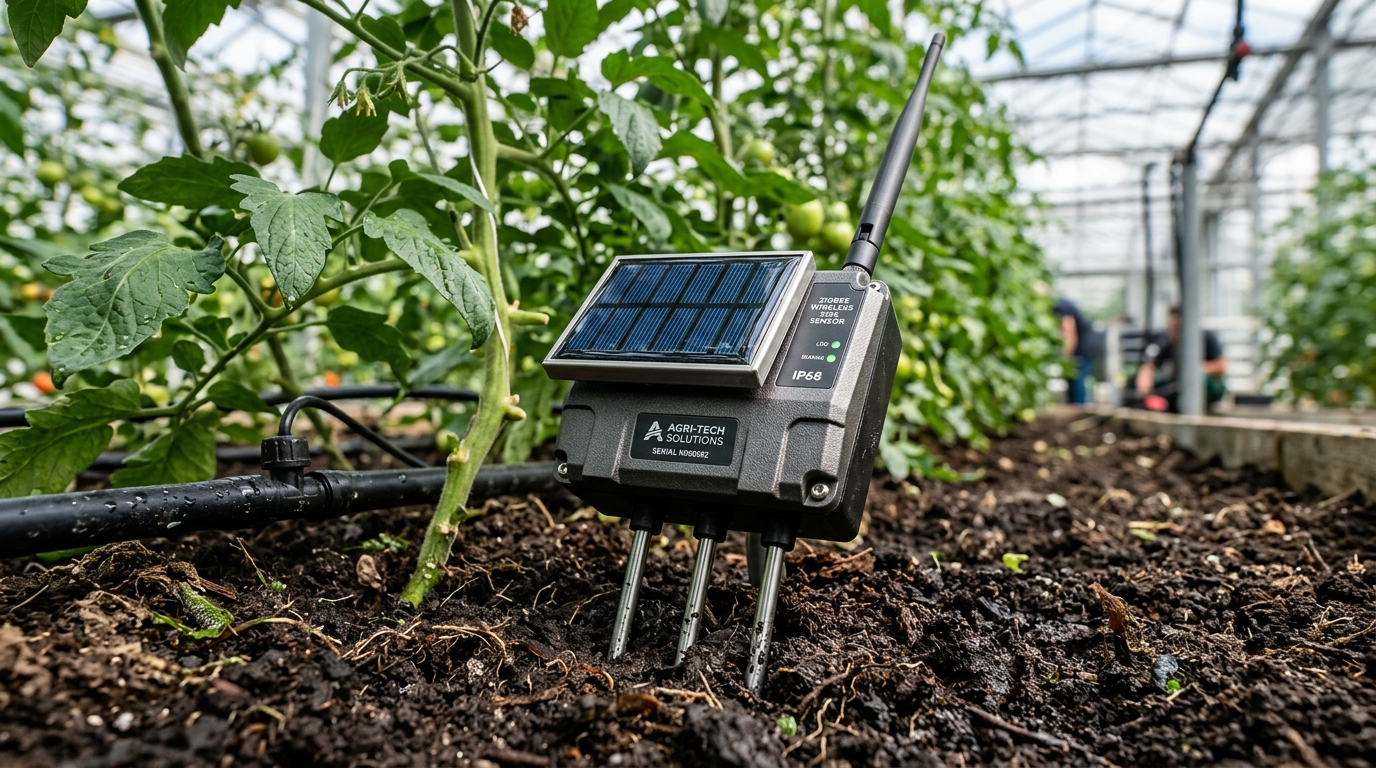
\includegraphics[width=0.88\textwidth]{figures/zigbee_soil_sensor_realistic.jpg}
    \caption{การติดตั้งหัววัดเซนเซอร์ดินอุตสาหกรรมแบบฝังลึกในแปลงเกษตรพร้อมโหนดรับส่งข้อมูล Zigbee}
    \label{fig:zigbee_soil_sensor}
\end{figure}

\section{การตรวจวัดสภาวะบรรยากาศและรังสีดวงอาทิตย์}

นอกเหนือจากสภาวะใต้ดินแล้ว สภาวะบรรยากาศเหนือดินมีอิทธิพลโดยตรงต่อกระบวนการสังเคราะห์ด้วยแสงและการคายน้ำของพืช การตรวจวัด \textbf{ความดันไอขาดดุล (Vapor Pressure Deficit หรือ VPD)}\index{VPD@VPD (ความดันไอขาดดุล)} ซึ่งคำนวณจากอุณหภูมิอากาศและความชื้นสัมพัทธ์ ถือเป็นตัวชี้วัดสำคัญที่สุดในการตัดสินใจเปิดปิดระบบพ่นหมอกและพัดลมระบายอากาศในโรงเรือน

ค่าความดันไอขาดดุลสามารถคำนวณได้จากสมการของเตเทนส์ (Tetens Equation)
\begin{equation}
    e_s(T) = 0.61078 \exp\left( \frac{17.27 T}{T + 237.3} \right) \quad \text{[kPa]}
\end{equation}
\begin{equation}
    \text{VPD} = e_s(T) \times \left(1 - \frac{\text{RH}}{100}\right) \quad \text{[kPa]}
\end{equation}
โดยที่ $e_s(T)$ คือความดันไออิ่มตัวที่อุณหภูมิ $T$ ในหน่วยองศาเซลเซียส และ $\text{RH}$ คือความชื้นสัมพัทธ์ในหน่วยเปอร์เซ็นต์

\begin{figure}[H]
    \centering
    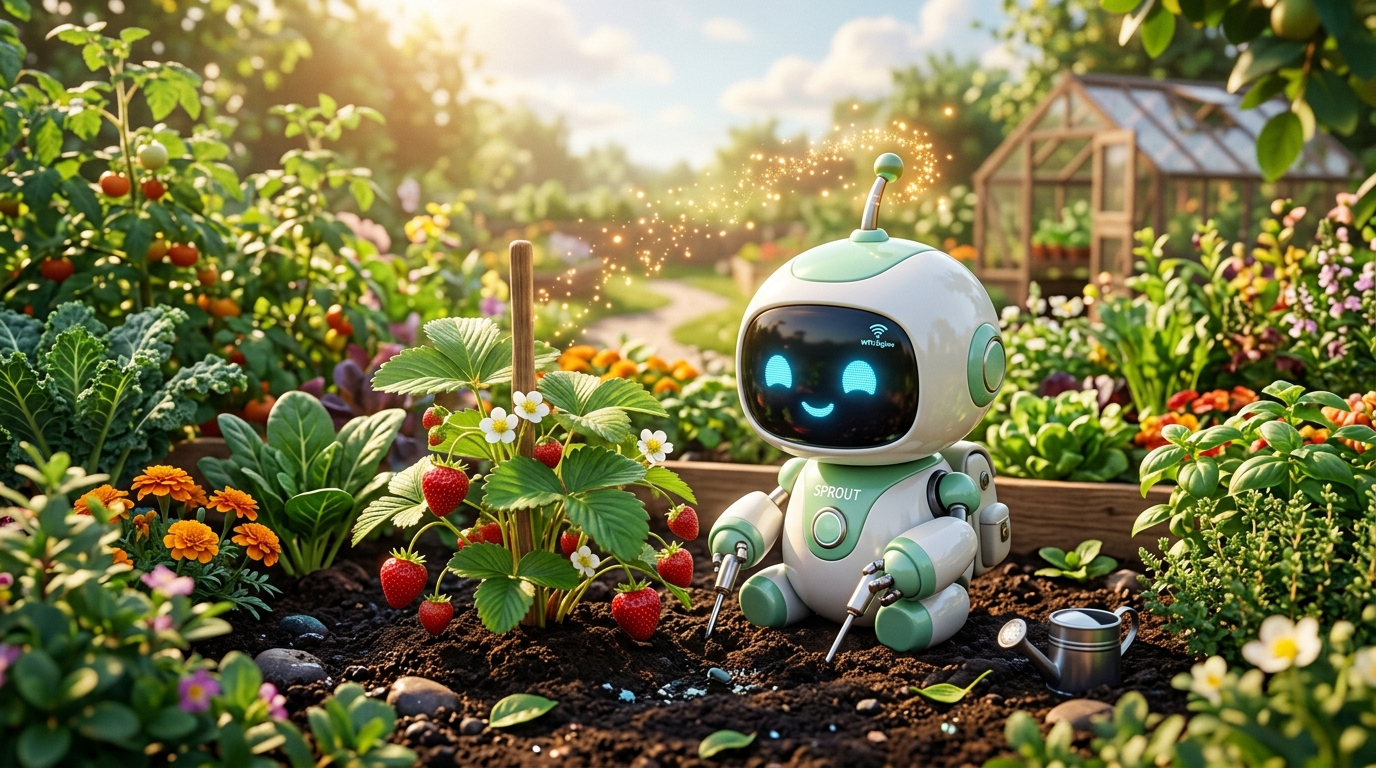
\includegraphics[width=0.88\textwidth]{figures/zigbee_sensor_pixar_3d.jpg}
    \caption{แบบจำลอง 3 มิติแสดงโครงสร้างสถาปัตยกรรมโหนดเซนเซอร์ Zigbee บูรณาการหัววัดดินและหัววัดสภาพอากาศ}
    \label{fig:zigbee_sensor_3d}
\end{figure}

\section{สถาปัตยกรรมสะพานสื่อสาร RS485 Modbus RTU สู่ Zigbee}

เนื่องจากเซนเซอร์ภาคสนามเกรดอุตสาหกรรมส่วนใหญ่ใช้พอร์ตสื่อสารแบบสายชนิด \textbf{อาร์เอส-485 (RS485)}\index{RS485@RS485} และโพรโทคอล \textbf{มอดบัส (Modbus RTU)}\index{Modbus RTU@Modbus RTU} เพื่อความทนทานต่อสัญญาณรบกวนแม่เหล็กไฟฟ้า การนำข้อมูลเข้าสู่โครงข่ายไร้สาย Zigbee จึงต้องอาศัยอุปกรณ์สะพานสื่อสาร (Bridge Node)

\begin{protocolbox}[โครงสร้างคำสั่งและการตรวจสอบความถูกต้องของ Modbus RTU]
การติดต่อสื่อสารแบบ Modbus RTU ทำงานในรูปแบบ Master-Slave โดยโหนด Zigbee จะทำหน้าที่เป็น Master ส่งคำสั่งแบบไบนารีไปยังเซนเซอร์โครงสร้างเฟรมประกอบด้วย
\begin{enumerate}
    \item \textbf{Slave Address (1 ไบต์)} ที่อยู่ประจำอุปกรณ์ เช่น 0x01
    \item \textbf{Function Code (1 ไบต์)} ฟังก์ชันการทำงาน เช่น 0x03 (Read Holding Registers)
    \item \textbf{Starting Address (2 ไบต์)} แอดเดรสเริ่มต้นของรีจิสเตอร์ที่ต้องการอ่าน
    \item \textbf{Number of Points (2 ไบต์)} จำนวนรีจิสเตอร์ที่ต้องการอ่าน เช่น 0x0007 (อ่าน 7 ตัว)
    \item \textbf{Cyclic Redundancy Check หรือ CRC-16 (2 ไบต์)} รหัสตรวจสอบความถูกต้องข้อมูลตามพหุนาม $x^{16} + x^{15} + x^2 + 1$
\end{enumerate}
\end{protocolbox}

\begin{table}[H]
\caption{ตัวอย่างผังรีจิสเตอร์ของหัววัดดินอุตสาหกรรม 7-in-1 Modbus RTU}
\label{tab:modbus_register_map}
\centering
\small
\begin{tabularx}{\textwidth}{c c c >{\raggedright\arraybackslash}X c}
\toprule
\textbf{Register Address} & \textbf{พารามิเตอร์} & \textbf{หน่วย} & \textbf{ตัวคูณสเกล (Scaling Factor)} & \textbf{ชนิดข้อมูล} \\
\midrule
0x0000 & ความชื้นดิน (Soil Moisture) & \% & 0.1 (เช่น ค่า 452 หมายถึง 45.2\%) & 16-bit Unsigned \\
0x0001 & อุณหภูมิดิน (Soil Temp) & $^\circ\text{C}$ & 0.1 (ค่าลบใช้ 2's Complement) & 16-bit Signed \\
0x0002 & การนำไฟฟ้า (Soil EC) & $\mu\text{S/cm}$ & 1 (เช่น ค่า 1250 หมายถึง 1250 $\mu\text{S/cm}$) & 16-bit Unsigned \\
0x0003 & ความเป็นกรดด่าง (Soil pH) & pH & 0.1 (เช่น ค่า 68 หมายถึง 6.8 pH) & 16-bit Unsigned \\
0x0004 & ไนโตรเจน (Nitrogen - N) & mg/kg & 1 & 16-bit Unsigned \\
0x0005 & ฟอสฟอรัส (Phosphorus - P) & mg/kg & 1 & 16-bit Unsigned \\
0x0006 & โพแทสเซียม (Potassium - K) & mg/kg & 1 & 16-bit Unsigned \\
\bottomrule
\end{tabularx}
\end{table}

\begin{warningbox}[ข้อควรระวังในการต่อวงจร RS485 ภาคสนาม]
การติดตั้งสายสัญญาณ RS485 ในแปลงเกษตรกรรมมีความเสี่ยงสูงต่อฟ้าผ่าและแรงดันเกินชั่วขณะ (Transient Voltage) วิศวกรต้องปฏิบัติตามข้อกำหนดดังนี้
\begin{enumerate}
    \item ใช้สายสัญญาณชนิดคู่บิดเกลียวพร้อมแผ่นชิลด์กันสัญญาณกวน (Shielded Twisted Pair หรือ STP) โดยต่อกราวด์แผ่นชิลด์ที่ฝั่งเกตเวย์เพียงจุดเดียว (Single-Point Grounding) เพื่อป้องกัน Ground Loop
    \item ติดตั้งตัวต้านทานต่อปลายสาย (Termination Resistor) ขนาด 120 โอห์ม ที่จุดปลายสุดของสายสัญญาณทั้งสองด้าน เพื่อป้องกันการสะท้อนของคลื่น
    \item ติดตั้งไดโอดป้องกันแรงดันเสิร์จ (TVS Diode) และวงจรตัดต่อกัลวานิก (Optocoupler / Digital Isolator) เพื่อป้องกันไม่ให้ไฟกระชากทำลายบอร์ดไมโครคอนโทรลเลอร์
\end{enumerate}
\end{warningbox}

\section{การเปรียบเทียบระหว่างโหนดสำเร็จรูปเชิงพาณิชย์และโหนดโอเพนซอร์ส}

\begin{table}[H]
\caption{การวิเคราะห์เปรียบเทียบโหนดเซนเซอร์สำเร็จรูปเชิงพาณิชย์และโหนดโอเพนซอร์ส}
\label{tab:commercial_vs_custom}
\centering
\small
\begin{tabularx}{\textwidth}{p{3.0cm} >{\raggedright\arraybackslash}X >{\raggedright\arraybackslash}X}
\toprule
\textbf{หัวข้อเปรียบเทียบ} & \textbf{โหนดสำเร็จรูปเชิงพาณิชย์ (Commercial)} & \textbf{โหนดปรับแต่งเอง (Custom ESP32-C6)} \\
\midrule
ความง่ายในการใช้งาน & เสียบใช้งานได้ทันที ผูกกับแอปพลิเคชันสำเร็จรูป & ต้องเขียนเฟิร์มแวร์และออกแบบวงจรพิมพ์ \\
ความยืดหยุ่น & ปรับแต่งแก้ไขโพรโทคอลไม่ได้ & ปรับอัลกอริทึมและเพิ่มเซนเซอร์ได้อิสระ \\
การผสานรวมระบบ & มักติดล็อกอยู่กับเซิร์ฟเวอร์ผู้ผลิต (Vendor Lock-in) & เปิดกว้าง เชื่อมต่อตรงสู่ MQTT / Home Assistant \\
ต้นทุนต่อหน่วย & ราคาสูง (3,500--8,000 บาทต่อชุด) & ราคาต่ำ (800--1,800 บาทต่อชุด) \\
การบำรุงรักษา & ต้องส่งศูนย์บริการซ่อม & วิศวกรประจำฟาร์มสามารถเปลี่ยนอะไหล่ได้ทันที \\
\bottomrule
\end{tabularx}
\end{table}

\clearpage

% ------------------------------------------------------------
% คำถามทบทวนท้ายบทที่ 2
% ------------------------------------------------------------
\section*{คำถามทบทวนท้ายบทที่ 2}
\addcontentsline{toc}{section}{คำถามทบทวนท้ายบทที่ 2}

\begin{enumerate}
    \item จงอธิบายความแตกต่างระหว่างการวัดความชื้นดินแบบ Frequency Domain Reflectometry (FDR) และ Time Domain Reflectometry (TDR) เหตุใดวิธี FDR จึงเป็นที่นิยมในโหนดเซนเซอร์ขนาดเล็ก
    \item ค่าความดันไอขาดดุล (Vapor Pressure Deficit หรือ VPD) มีความสัมพันธ์กับอัตราการคายน้ำของพืชอย่างไร และเหตุใดการวัดเพียงค่าอุณหภูมิและความชื้นสัมพัทธ์แยกกันจึงไม่เพียงพอต่อการควบคุมโรงเรือนอัจฉริยะ
    \item กำหนดให้เซนเซอร์ดิน Modbus RTU ส่งข้อมูลไบนารีค่าความชื้น 0x01B8 และอุณหภูมิ 0x0104 จงคำนวณค่าจริงในหน่วยเปอร์เซ็นต์และองศาเซลเซียสตามผังรีจิสเตอร์ในตารางที่ \ref{tab:modbus_register_map}
    \item เหตุใดการต่อสายสัญญาณ RS485 ในระยะทางไกลจึงจำเป็นต้องติดตั้งตัวต้านทาน 120 โอห์มที่ปลายสาย หากไม่ติดตั้งจะส่งผลกระทบต่อรูปสัญญาณอย่างไร
    \item ในการออกแบบโหนดเซนเซอร์ดินที่ติดตั้งกลางแจ้ง จงอธิบายมาตรการป้องกันความชื้นและฝุ่นละอองตามมาตรฐาน IP68 และการป้องกันแรงดันกระชากจากฟ้าผ่า
\end{enumerate}

\clearpage
